\documentclass[11pt]{article}
\usepackage{euscript}

\usepackage{amsmath}
\usepackage{amsthm}
\usepackage{amssymb}
\usepackage{epsfig}
\usepackage{xspace}
\usepackage{color}
\usepackage{url}

%%%%%%%%%%%%%%%%%%%%%%%%%%%%%%%%%
\setlength{\textheight}{9in}
\setlength{\topmargin}{-0.600in}
\setlength{\headheight}{0.2in}
\setlength{\headsep}{0.250in}
\setlength{\footskip}{0.5in}
\flushbottom
\setlength{\textwidth}{6.5in}
\setlength{\oddsidemargin}{0in}
\setlength{\evensidemargin}{0in}
\setlength{\columnsep}{2pc}
\setlength{\parindent}{1em}
%%%%%%%%%%%%%%%%%%%%%%%%%%%%%%%%%


\newcommand{\eps}{\varepsilon}

\renewcommand{\c}[1]{\ensuremath{\EuScript{#1}}}
\renewcommand{\b}[1]{\ensuremath{\mathbb{#1}}}
\newcommand{\s}[1]{\textsf{#1}}

\newcommand{\E}{\textbf{\textsf{E}}}
\renewcommand{\Pr}{\textbf{\textsf{Pr}}}

\title{Homework Form for Data Mining
\footnote{\s{CS 6955 Data Mining; \;\; Spring 2012 \hfill
Instructor: Jeff M. Phillips, University of Utah}
}
}
\author{Alex Clemmer}

\begin{document}
\maketitle





%%%%%%%%%%%%%%%%%%%%%%%%%%%%%%%%%%%%%%%%%%%%%%%%%%%%
%%%%%%%%%%%%%%%%%%%%%%%%%%%%%%%%%%%%%%%%%%%%%%%%%%%%
%%%%%%%%%%%%%%%%%%%%%%%%%%%%%%%%%%%%%%%%%%%%%%%%%%%%
\section*{Overview}

This is a sample latex file to use for completing assignments.  This particular file is not required.  In fact, there are many cool ways to spruce up this plain look.  Feel free to use them.  

\section*{Q1: Birthday ``Paradox"}

\paragraph*{A:} For domain $n = 1000$, it took 58 random trials.

\paragraph*{B:} Please see figure \ref{fig:cdp1}.

\begin{figure}[h]
\centering{
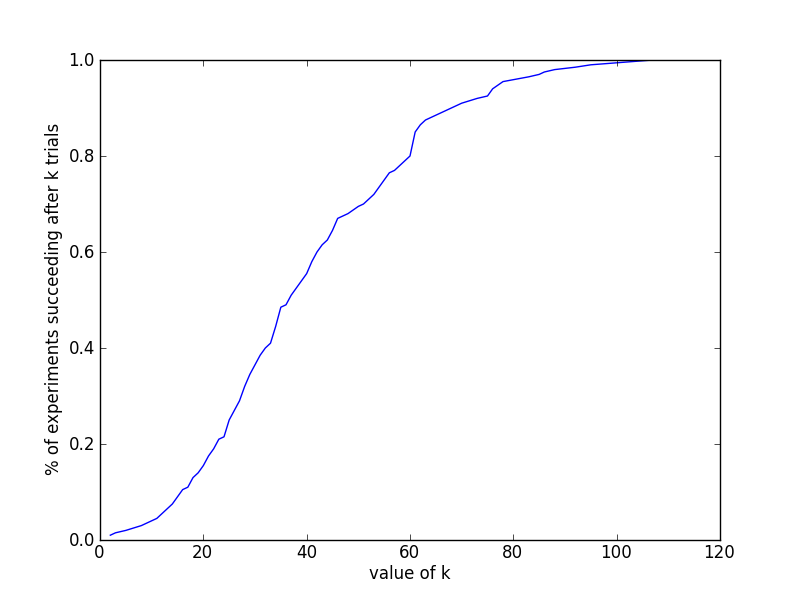
\includegraphics[width=.6\linewidth]{fig1.png}
}
\caption{The \% of experiments requiring $k$ tests before collision, plotted as a function of $k$.}
\label{fig:cdp1}
\end{figure}

\paragraph*{C:} For some $m = 200$ random variables $X_1 \ldots X_m$ representing the outcomes of $m$ random repetitions of the experiment, the expected value $\E[\vec{X}] = 38.005$

\paragraph*{D:} 

I check uniqueness using a bit vector of length $n$, where each place is 0 if we haven't seen the corresponding element before, and is 1 if we have. We use a Mersenne Twister as the random number generator. We run the experiment, continuously checking if the generated number corresponds to an already-filled bit in the bit vector.

As long as this bit vector fits in memory, it should scale pretty well. Experimentally this bears out well: in figure \ref{fig:runningtimes1}, we show experimentally that, for $n = 1,000,000$, even when we increase $m$ by orders of 10 starting at $m=10$, the algorithm still runs in roughly linear time.


\begin{figure}[h]
\centering{
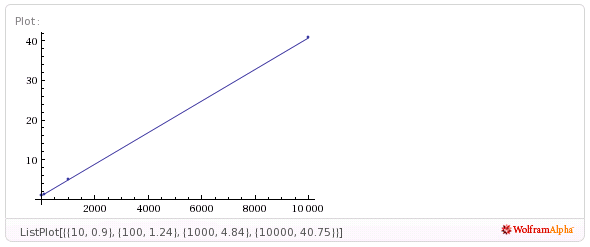
\includegraphics[width=.6\linewidth]{blowup.png}
}
\caption{The running time ($x$-axis) increases by successive powers of 10; the $y$-axis denotes the running time of seconds it took to complete.}
\label{fig:runningtimes1}
\end{figure}

\section*{Q2: Coupon Collectors}

\paragraph*{A:} For the domain $n = 60$, the required trials $k = 198$.

\paragraph*{B:} As we can see in figure \ref{fig:hist}, the highest bar was pinged 10 times.

\begin{figure}[h]
\centering{
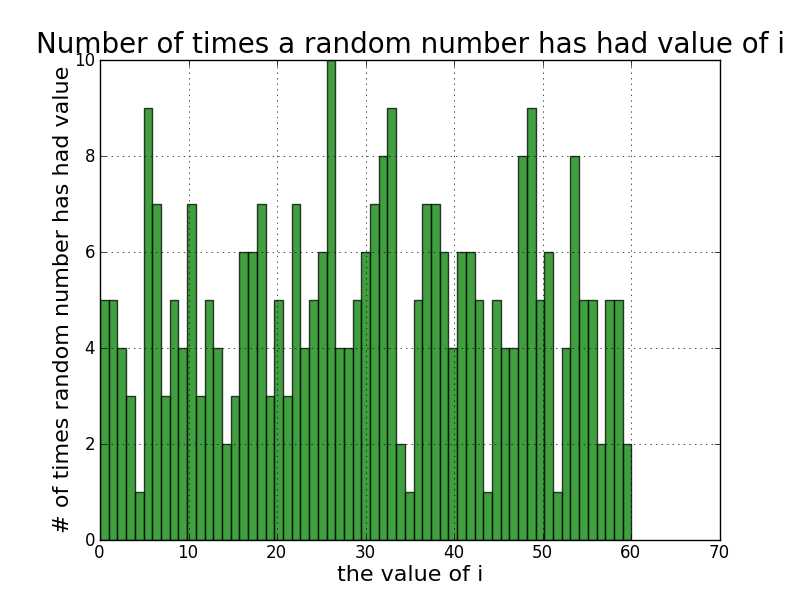
\includegraphics[width=.6\linewidth]{fig3.png}
}
\caption{The number of times a random number ends up with value $i$.}
\label{fig:hist}
\end{figure}

\paragraph*{C:} Please see figure \ref{fig:cdp2}.

\begin{figure}[h]
\centering{
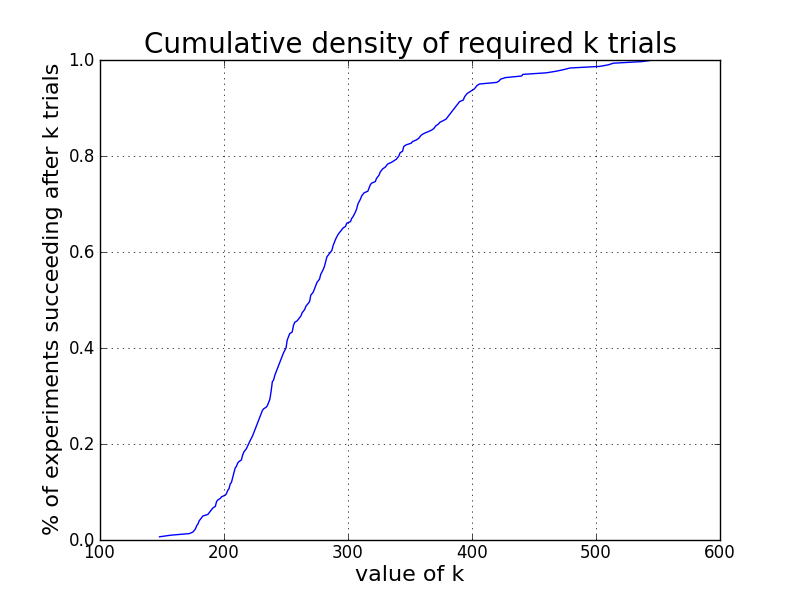
\includegraphics[width=.6\linewidth]{fig4.png}
}
\caption{The number of times a random number ends up with value $i$.}
\label{fig:cdp2}
\end{figure}

\paragraph*{D:} For some $m = 300$ random variables $X_1 \ldots X_m$ representing the outcomes of $m$ random repetitions of the experiment, the expected value $\E[\vec{X}] = 283.61$

\paragraph*{E:} Our ``basic" algorithm again used an $n$-length bit vector to check for collisions, but this time we also kept track of the number of unique elements; when this number reaches $n$, we halt the algorithm. We again used a Mersenne Twister for random number generation.

This is not going to scale as well. In figure \ref{fig:runningtimes2}, we increase $n$ by orders of 10, for constant $m = 300$. Note that it is larger than linear. The main reason is that the expected number of times we need to generate a number before we have generated every number in a domain of $n$ is going to be asymptotically much larger than linear with respect to $n$.

\begin{figure}[h]
\centering{
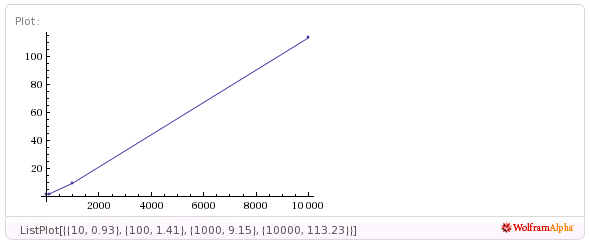
\includegraphics[width=.6\linewidth]{blowup2.png}
}
\caption{The running time ($x$-axis) increases by successive powers of 10; the $y$-axis denotes the running time of seconds it took to complete.}
\label{fig:runningtimes2}
\end{figure}

How much this can be sped up depends on what the real bottleneck is. If the real bottleneck is generating the random numbers sequentially (and I suspect it is), then you can probably improve performance by parallelizing the random number generation. You might begin, for example, by firing off some $t$ different ``mapper" threads, each of which is constantly generating numbers from Mersenne Twister, simply dumping them to a common place (\textit{e.g.}, standard out). You could then employ a single ``reducer" thread, whose only job is to simply check whether we've seen a particular number against the bit vector.

Notably, this does not completely eliminate the runtime issues. What it \textit{does} do is shift the bottleneck to communication. It's not a solution to the problem; you're really just switching one bad problem for another.


\section*{Q3: Analysis}

\textbf{A:} The explicit formula for $n = 1000$ is

\begin{eqnarray*}
1-(1-\cfrac{1}{1000})^{k \choose 2} = 1/2
\end{eqnarray*}

Assuming $k$ is real, we can reduce to:

\begin{eqnarray*}
1 - ((\cfrac{3}{10})^{k^2-k})^{3/2} \sqrt{37^{k^2-k}} = 1/2
\end{eqnarray*}

This is polynomial equation which we can solve the usual way, giving us:

\begin{eqnarray*}
k = 37.727
\end{eqnarray*}


\textbf{B:} The explicit formula for $n = 60$ is a straightforward calculation. I actually got my formula from Wikipedia, since the formulation in the notes gave me a weird result. Their formulation is also convincing (I think that the series analysis in the notes is wrong). Anyway, it gives us a much closer result to empirical truth:

\begin{eqnarray*}
k & = & n \log n + \gamma n + \cfrac{1}{2} + C_1 \\
& = & (1 + \gamma) 60 \log 60 \\
& \approx & 280.7806
\end{eqnarray*}




\end{document}
